\documentclass[10pt,aspectratio=169]{beamer}

% --- Theme & Colors ---
\usetheme{Madrid}
\usecolortheme{whale}

\definecolor{mainblue}{RGB}{0,73,131}
\definecolor{darkblue}{RGB}{0,47,95}
\definecolor{accentblue}{RGB}{70,130,180}
\definecolor{lightgray}{RGB}{240,240,240}

\setbeamercolor{structure}{fg=mainblue}
\setbeamercolor{palette primary}{bg=mainblue,fg=white}
\setbeamercolor{palette secondary}{bg=darkblue,fg=white}
\setbeamercolor{palette tertiary}{bg=darkblue,fg=white}
\setbeamercolor{frametitle}{bg=mainblue,fg=white}
\setbeamercolor{title}{bg=mainblue,fg=white}
\setbeamercolor{block title}{bg=mainblue,fg=white}
\setbeamercolor{block body}{bg=lightgray,fg=black}
\setbeamercolor{block title alerted}{bg=red!70!black,fg=white}
\setbeamercolor{block title example}{bg=accentblue,fg=white}
\setbeamercolor{block body example}{bg=lightgray,fg=black}

\setbeamertemplate{navigation symbols}{}
\setbeamertemplate{footline}{%
  \leavevmode%
  \hbox{%
    \begin{beamercolorbox}[wd=.33\paperwidth,ht=2.5ex,dp=1ex,center]{palette primary}%
      \usebeamerfont{author in head/foot}\insertshortauthor
    \end{beamercolorbox}%
    \begin{beamercolorbox}[wd=.34\paperwidth,ht=2.5ex,dp=1ex,center]{palette secondary}%
      \usebeamerfont{title in head/foot}\insertshorttitle
    \end{beamercolorbox}%
    \begin{beamercolorbox}[wd=.33\paperwidth,ht=2.5ex,dp=1ex,right]{palette tertiary}%
      \insertframenumber{} / \inserttotalframenumber\hspace*{2ex}
    \end{beamercolorbox}%
  }%
}

% --- Packages ---
\usepackage{amsmath,amssymb,amsthm}
\usepackage{graphicx}
\usepackage{tikz}
\usetikzlibrary{arrows.meta,positioning,calc,decorations.pathreplacing}
\usepackage{hyperref}
\usepackage{booktabs}
\usepackage{algorithm2e}
\usepackage{bm}

\graphicspath{{pics/}}

% --- Meta ---
\title[MC I: Classical Algorithms]{MonteCarlo: From Classic to Quantum\\[0.3em]
\large I. Classical MarkovChain Monte Carlo Algorithms}
\author[YK. Xu]{Yongkang Xu}
\institute[ZJU]{Center of Correlated Matter, Zhejiang University}
\date{\today}

\begin{document}

% --- Title ---
\begin{frame}
  \titlepage
\end{frame}

% --- Outline ---
\begin{frame}{Outline}
  \tableofcontents
\end{frame}

% ============================================================
\section{Motivation: TbCo$_2$ and the Kondo-Ising Model}
% ============================================================

\begin{frame}{TbCo$_2$: A Ferrimagnetic Laves Phase Compound}
  \begin{columns}[T]
    \column{0.5\textwidth}
    \begin{itemize}
      \item TbCo$_2$ crystallizes in the \textbf{cubic C15 Laves phase} structure
      \item Co atoms form a network of corner-sharing tetrahedra
      \item Tb occupies the larger interstitial sites
      \item Ferrimagnetic order: Tb moments ($\sim 9\,\mu_B$) and Co moments ($\sim 1\,\mu_B$) couple \emph{antiparallel}
    \end{itemize}
    \vspace{0.3em}
    {\footnotesize Ref: Applied Physics Letters \textbf{121}, 232404 (2022)}
    \column{0.5\textwidth}
    \centering
    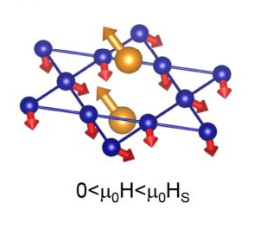
\includegraphics[width=0.85\textwidth]{TbCo2.png}\\[2pt]
    {\footnotesize Non-collinear ferrimagnetic structure\\under intermediate field $0 < \mu_0 H < \mu_0 H_s$}
  \end{columns}
\end{frame}

\begin{frame}{Crystal Structure: Co Kagome Sublattice}
  \begin{columns}[T]
    \column{0.5\textwidth}
    \begin{itemize}
      \item In certain crystallographic planes, Co atoms form a \textbf{kagome lattice}
      \item Tb atoms sit on a separate diamond-cubic sublattice
      \item The interplay of two magnetic sublattices gives rise to rich physics:
        \begin{itemize}
          \item Anomalous Hall effect
          \item Topological Hall effect
          \item Non-coplanar spin textures
        \end{itemize}
    \end{itemize}
    \column{0.5\textwidth}
    \centering
    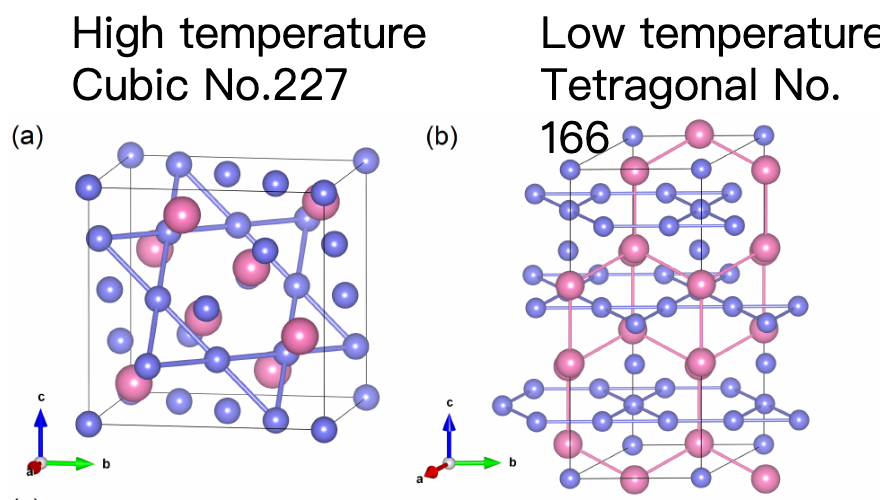
\includegraphics[width=0.85\textwidth]{TbCo2Lattice.png}\\[2pt]
    {\footnotesize C15 Laves phase unit cell\\(blue: Co, pink: Tb)}
  \end{columns}
\end{frame}

\begin{frame}{Anomalous Transport Properties of TbCo$_2$}
  \begin{columns}[T]
    \column{0.45\textwidth}
    \begin{itemize}
      \item Non-linear Hall resistivity $\rho_{xy}$ — characteristic of \textbf{Anomalous Hall Effect} (AHE)
      \item \textbf{Topological Hall Effect} (THE) signal observed near $T_C = 232\,$K
      \item Sharp negative magnetoresistance peak at $T_C$
      \item These signatures point to a non-trivial spin--charge coupling mechanism
    \end{itemize}
    \column{0.55\textwidth}
    \centering
    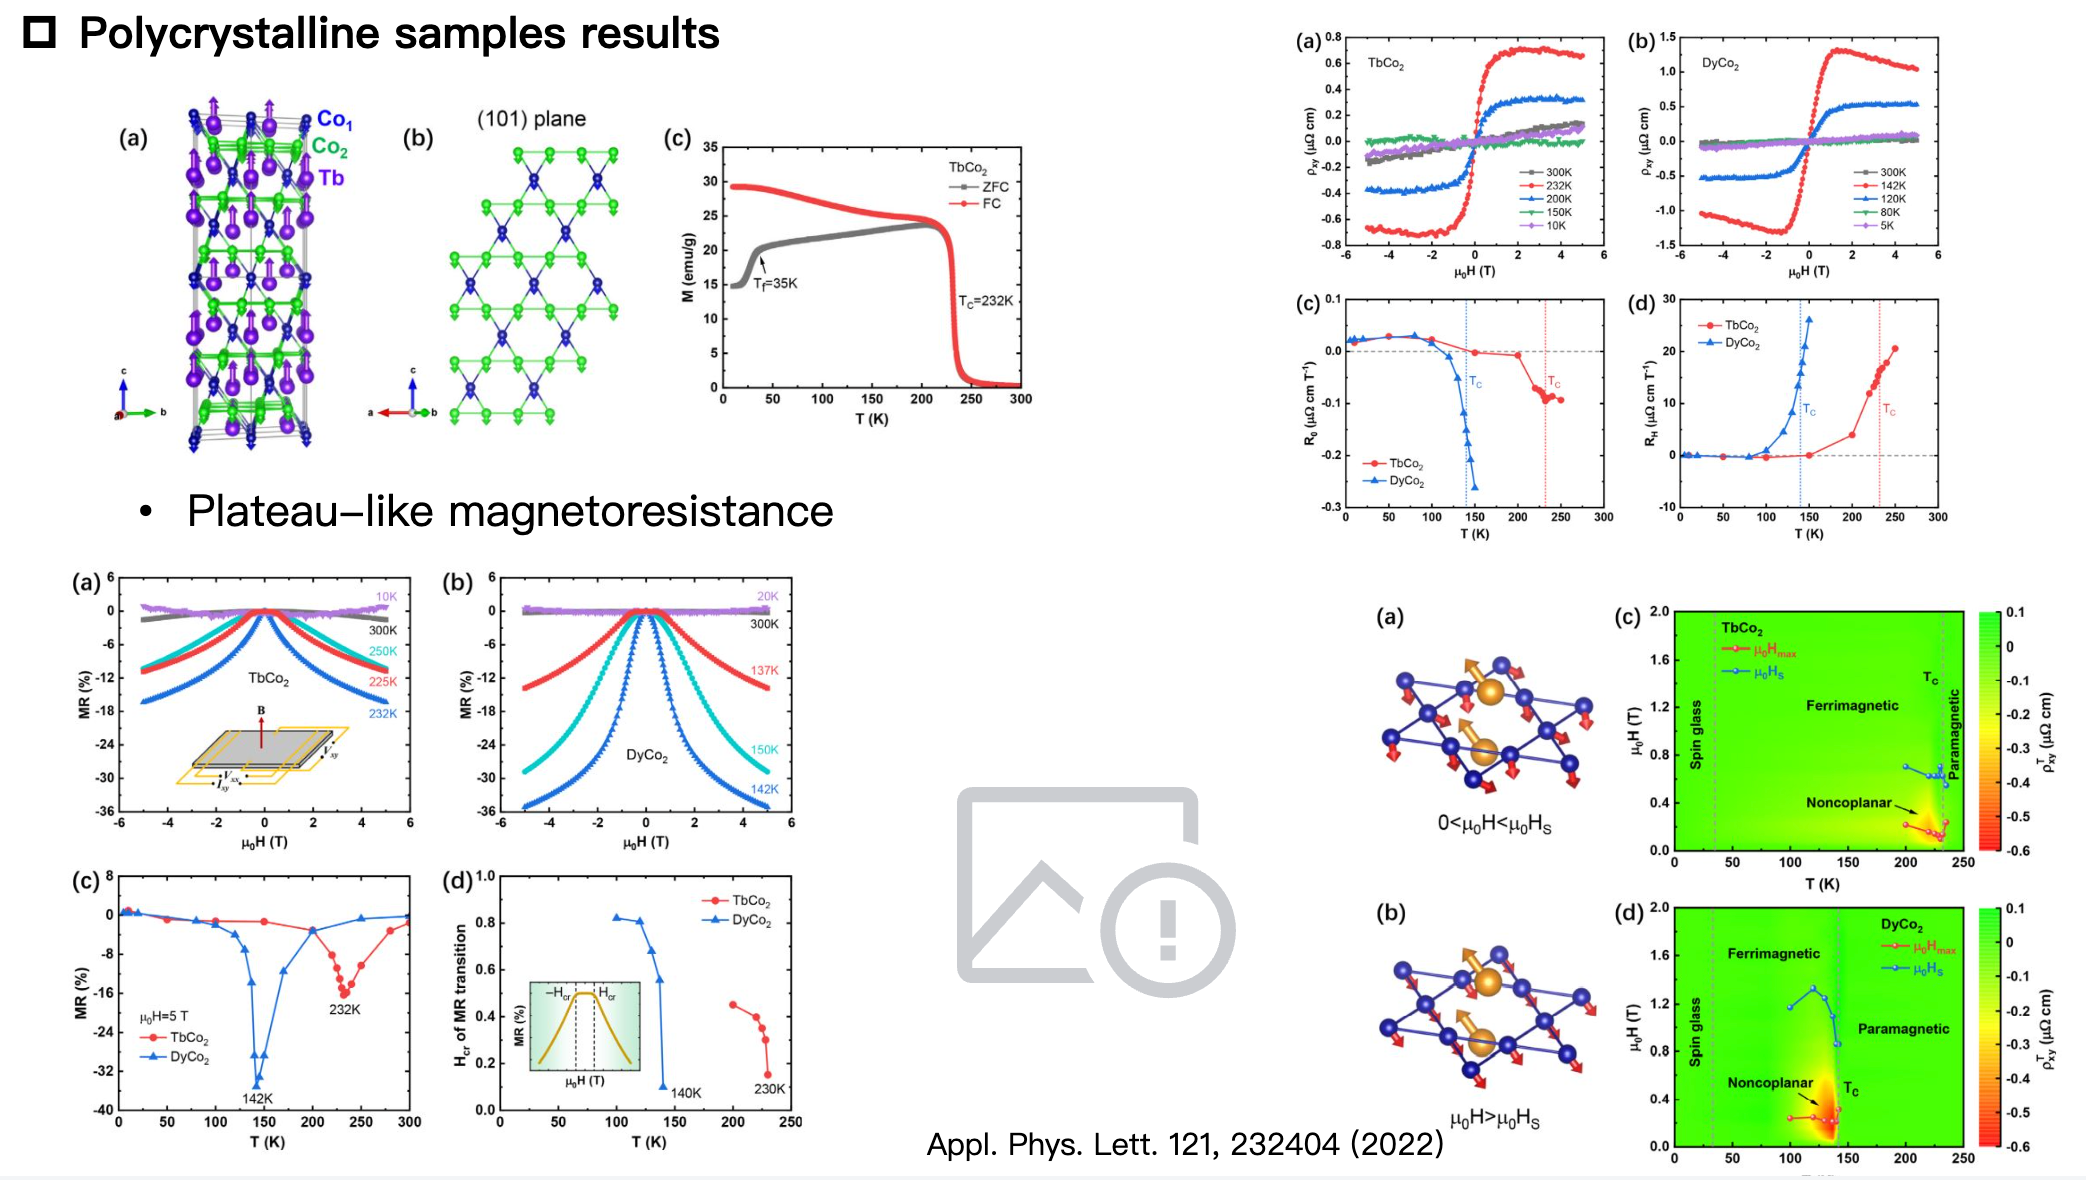
\includegraphics[width=\textwidth]{TbCo2_transport_properties.png}\\[2pt]
    {\footnotesize Transport measurements on polycrystalline TbCo$_2$\\(Appl.\ Phys.\ Lett.\ \textbf{121}, 232404)}
  \end{columns}
\end{frame}

\begin{frame}{From TbCo$_2$ to the Kondo-Ising Model}
  \begin{columns}[c]
    \column{0.48\textwidth}
    \centering
    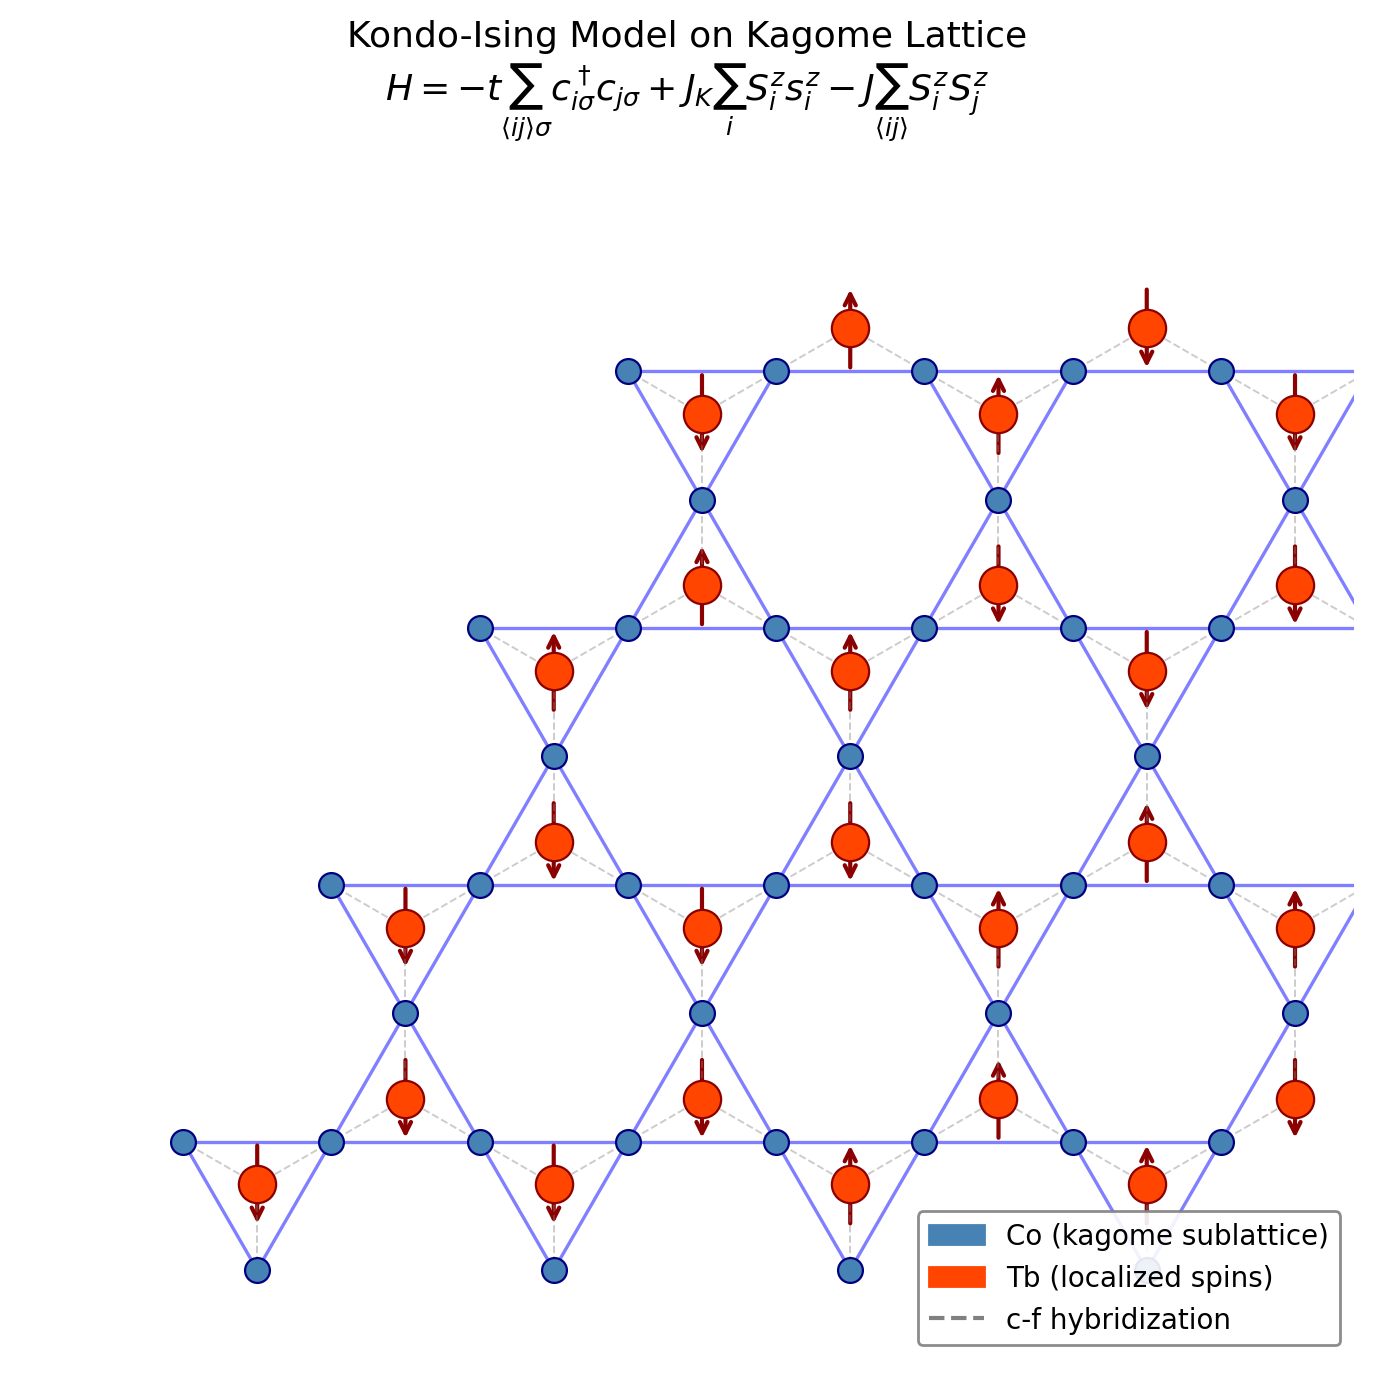
\includegraphics[width=\textwidth,height=0.78\textheight,keepaspectratio]{kagome_kondo_ising.png}\\[2pt]
    {\footnotesize 2D kagome lattice view}
    \column{0.48\textwidth}
    \centering
    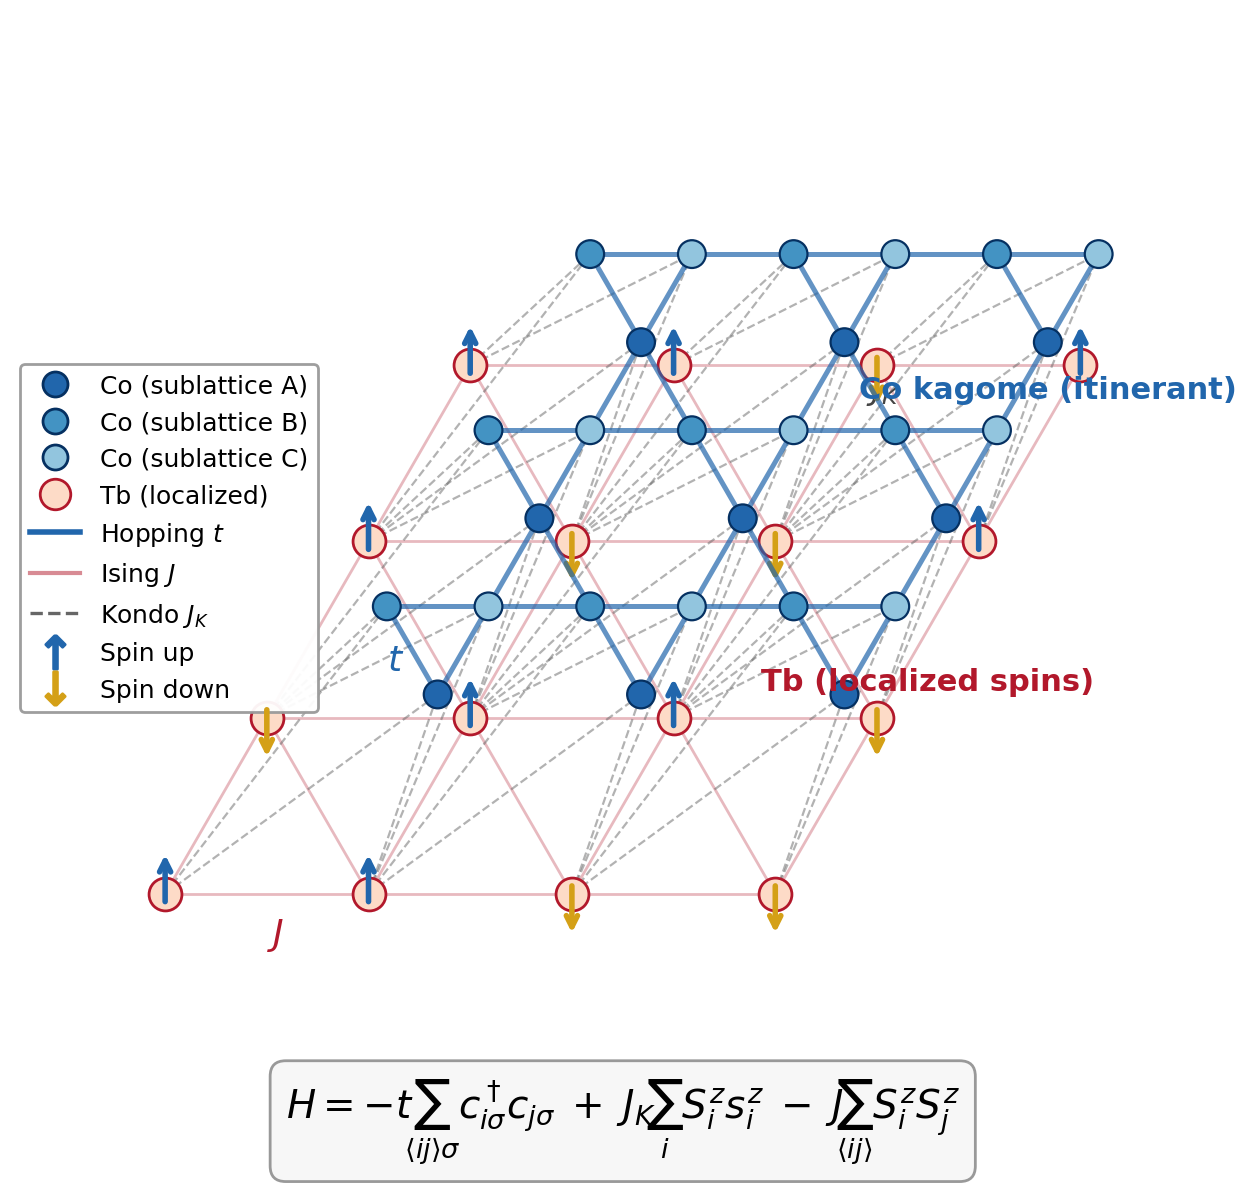
\includegraphics[width=\textwidth,height=0.78\textheight,keepaspectratio]{kagome_kondo_ising_v2.png}\\[2pt]
    {\footnotesize Isometric bilayer view}
  \end{columns}
\end{frame}

\begin{frame}{Kondo-Ising Model: Hamiltonian}
  \begin{block}{Kondo-Ising Hamiltonian}
    \vspace{-0.5em}
    \[
      H = \underbrace{-t \sum_{\langle ij\rangle,\sigma} c_{i\sigma}^\dagger c_{j\sigma}}_{\text{itinerant electrons (Co)}}
        + \underbrace{J_K \sum_i S_i^z\, s_i^z}_{\text{Kondo coupling}}
        - \underbrace{J \sum_{\langle ij\rangle} S_i^z\, S_j^z}_{\text{Ising interaction (Tb)}}
    \]
  \end{block}
  \vspace{0.5em}
  \begin{itemize}
    \item \textbf{Assumption:} c--f hybridization is weak $\rightarrow$ project onto Ising anisotropy limit
    \item The model separates naturally into two parts:
      \begin{enumerate}
        \item \textbf{Itinerant electron part} (Co): temperature enters only through Fermi--Dirac smearing
        \item \textbf{Localized spin part} (Tb): treated as a classical Ising system via \textbf{Monte Carlo}
      \end{enumerate}
    \item The localized spins act as an effective \textbf{mean field} on itinerant electrons
  \end{itemize}
  \vspace{0.3em}
  {\footnotesize Refs: W.-W.\ Yang \emph{et al.}, PRB \textbf{100}, 045148 (2019); PRB \textbf{102}, 195141 (2020); PRB \textbf{104}, 165146 (2021)}
\end{frame}

\begin{frame}{Roadmap: Why Classical Monte Carlo?}
  \begin{columns}[T]
    \column{0.55\textwidth}
    \begin{itemize}
      \item The Kondo-Ising model requires \textbf{thermal sampling} of the localized spin configuration $S^z_i$ at each temperature
      \item This is a \textbf{classical} Monte Carlo problem:
        \begin{itemize}
          \item Configuration space: $\{S^z_i = \pm 1\}$
          \item Boltzmann weight: $e^{-\beta E[\{S^z\}]}$
        \end{itemize}
      \item \textbf{This lecture:} classical MC algorithms (Metropolis, SW, Wolff)
      \item \textbf{Later lectures:} apply to Kondo-Ising; extend to quantum MC
    \end{itemize}
    \column{0.45\textwidth}
    \centering
    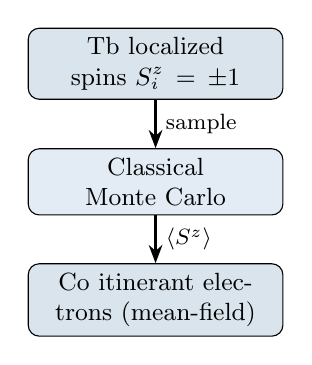
\begin{tikzpicture}[
      box/.style={draw, rounded corners, minimum width=3cm, minimum height=0.8cm,
                  text centered, font=\small, text width=3cm, align=center},
      arr/.style={-{Stealth}, thick}
    ]
      \node[box, fill=mainblue!15] (tb) at (0,3) {Tb localized spins $S^z_i = \pm 1$};
      \node[box, fill=accentblue!15] (mc) at (0,1.5) {Classical Monte Carlo};
      \node[box, fill=mainblue!15] (co) at (0,0) {Co itinerant electrons (mean-field)};
      \draw[arr] (tb) -- (mc) node[midway, right, font=\footnotesize] {sample};
      \draw[arr] (mc) -- (co) node[midway, right, font=\footnotesize] {$\langle S^z \rangle$};
    \end{tikzpicture}
  \end{columns}
\end{frame}

% ============================================================
\section{Monte Carlo Fundamentals}
% ============================================================

\begin{frame}{Monte Carlo Sampling: The Core Idea}
  \begin{columns}[T]
    \column{0.48\textwidth}
    \begin{itemize}
      \item \textbf{Goal:} compute thermal expectation values
        \[
          \langle A \rangle = \sum_{\{S\}} A[\{S\}]\;\pi[\{S\}]
        \]
      \item Boltzmann distribution:
        \[
          \pi[\{S\}] = \frac{e^{-\beta \mathcal{H}[\{S\}]}}{Z},
          \quad Z = \sum_{\{S\}} e^{-\beta \mathcal{H}[\{S\}]}
        \]
      \item \textbf{Problem:} $Z$ is intractable — combinatorial explosion of configurations
      \item \textbf{Solution:} construct a Markov chain that visits configurations with frequency $\propto \pi$
    \end{itemize}
    \column{0.50\textwidth}
    \centering
    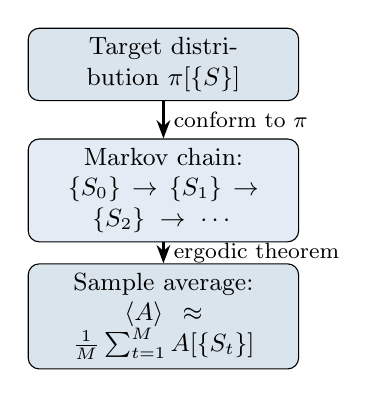
\begin{tikzpicture}[
      box/.style={draw, rounded corners, minimum width=3.2cm, minimum height=0.8cm,
                  text centered, font=\small, text width=3.2cm, align=center},
      arr/.style={-{Stealth}, thick}
    ]
      \node[box, fill=mainblue!15] (dist) at (0,3.6) {Target distribution $\pi[\{S\}]$};
      \node[box, fill=accentblue!15] (chain) at (0,2.0) {Markov chain:\\$\{S_0\} \to \{S_1\} \to \{S_2\} \to \cdots$};
      \node[box, fill=mainblue!15] (est) at (0,0.4) {Sample average:\\$\langle A \rangle \approx \frac{1}{M}\sum_{t=1}^{M} A[\{S_t\}]$};
      \draw[arr] (dist) -- (chain) node[midway, right, font=\footnotesize] {conform to $\pi$};
      \draw[arr] (chain) -- (est) node[midway, right, font=\footnotesize] {ergodic theorem};
    \end{tikzpicture}
  \end{columns}
\end{frame}

\begin{frame}{A Word on Computer Random Numbers}
  \begin{columns}[T]
    \column{0.45\textwidth}
    \begin{itemize}
      \item Computers generate \textbf{pseudo-random} numbers — deterministic sequences determined by a \textbf{seed}
      \item Advantage: fully reproducible simulations
      \item Caveat: long-range correlations may introduce bias
      \item Different seeds $\rightarrow$ different trajectories through configuration space
    \end{itemize}
    \vspace{0.5em}
    {\small \textit{Whether an MC algorithm is stable and how to characterize its trajectory will be discussed in Lecture~2.}}
    \column{0.53\textwidth}
    \centering
    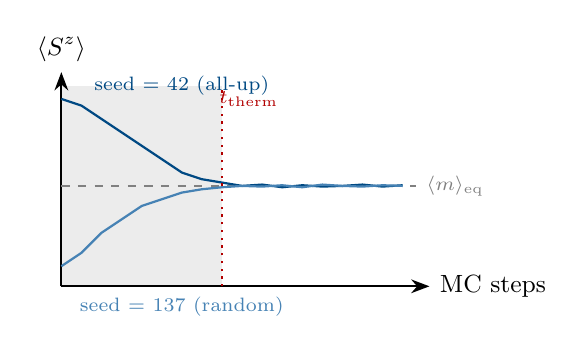
\begin{tikzpicture}[scale=0.85]
      % Thermalization shading (drawn first so tracks/labels render on top)
      \fill[gray!15] (0,0) rectangle (2.4,3.0);
      % Axes
      \draw[-{Stealth}, thick] (0,0) -- (5.5,0) node[right, font=\small] {MC steps};
      \draw[-{Stealth}, thick] (0,0) -- (0,3.2) node[above, font=\small] {$\langle S^z \rangle$};
      % Target line
      \draw[dashed, gray, thick] (0,1.5) -- (5.3,1.5) node[right, font=\scriptsize] {$\langle m \rangle_{\mathrm{eq}}$};
      % Track 1: all-up start
      \draw[thick, mainblue]
        (0,2.8) -- (0.3,2.7) -- (0.6,2.5) -- (0.9,2.3) -- (1.2,2.1)
        -- (1.5,1.9) -- (1.8,1.7) -- (2.1,1.6) -- (2.4,1.55)
        -- (2.7,1.5) -- (3.0,1.52) -- (3.3,1.48) -- (3.6,1.51)
        -- (3.9,1.49) -- (4.2,1.50) -- (4.5,1.52) -- (4.8,1.49) -- (5.1,1.51);
      \node[font=\scriptsize, mainblue] at (1.8,3.0) {seed = 42 (all-up)};
      % Track 2: random start
      \draw[thick, accentblue]
        (0,0.3) -- (0.3,0.5) -- (0.6,0.8) -- (0.9,1.0) -- (1.2,1.2)
        -- (1.5,1.3) -- (1.8,1.4) -- (2.1,1.45) -- (2.4,1.48)
        -- (2.7,1.50) -- (3.0,1.49) -- (3.3,1.51) -- (3.6,1.48)
        -- (3.9,1.52) -- (4.2,1.50) -- (4.5,1.49) -- (4.8,1.51) -- (5.1,1.50);
      \node[font=\scriptsize, accentblue] at (1.8,-0.3) {seed = 137 (random)};
      % Thermalization boundary
      \draw[dotted, red!70!black, thick] (2.4,0) -- (2.4,3.0);
      \node[font=\scriptsize, red!70!black] at (2.8,2.8) {$t_{\mathrm{therm}}$};
    \end{tikzpicture}
  \end{columns}
\end{frame}

\begin{frame}{Two Conditions for Correct Sampling}
  \begin{columns}[T]
    \column{0.53\textwidth}
    A Markov chain sampler must satisfy two conditions to converge to the target distribution $\pi$:
    \begin{block}{1.\ Detailed Balance}
      \vspace{-0.5em}
      \[
        W(A \to B)\;\pi(A) = W(B \to A)\;\pi(B)
      \]
      \vspace{-0.8em}
      {\small Equivalently: $\frac{W(A \to B)}{W(B \to A)} = e^{-\beta(E_B - E_A)}$\\[4pt]
      $\Longrightarrow$ $\pi$ is a \textbf{stationary distribution} of the chain.}
    \end{block}
    \begin{block}{2.\ Ergodicity}
      \vspace{-0.3em}
      {\small Every configuration is reachable from any other in finitely many steps:
      \[
        \forall\, A,\,B:\;\exists\, n \geq 1,\;\mathrm{Prob}(A \xrightarrow{n} B) > 0
      \]
      \vspace{-0.5em}
      $\Longrightarrow$ the stationary distribution is \textbf{unique}.}
    \end{block}

    \column{0.45\textwidth}
    \begin{exampleblock}{Why They Suffice}
      \begin{enumerate}\small
        \item Detailed balance $\Rightarrow$ $\pi$ is a \textbf{fixed point}
        \item Ergodicity $\Rightarrow$ fixed point is \textbf{unique}
        \item Together $\Rightarrow$ chain converges to $\pi$ from \emph{any} starting state
      \end{enumerate}
    \end{exampleblock}
    \vspace{0.5em}
    \centering
    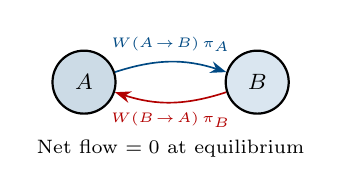
\begin{tikzpicture}[
      nd/.style={circle, draw, thick, minimum size=0.8cm, font=\footnotesize},
      arr/.style={-{Stealth}, semithick}
    ]
      \node[nd, fill=mainblue!20] (A) at (0,0) {$A$};
      \node[nd, fill=accentblue!20] (B) at (2.2,0) {$B$};
      \draw[arr, bend left=18, mainblue] (A) to
        node[above, font=\tiny] {$W(A\!\to\!B)\,\pi_A$} (B);
      \draw[arr, bend left=18, red!70!black] (B) to
        node[below, font=\tiny] {$W(B\!\to\!A)\,\pi_B$} (A);
      \node[font=\scriptsize] at (1.1,-0.85) {Net flow $= 0$ at equilibrium};
    \end{tikzpicture}
  \end{columns}
\end{frame}

\begin{frame}{Thermalization: When Can We Start Measuring?}
  \begin{columns}[T]
    \column{0.52\textwidth}
    \begin{block}{Thermalization (Burn-in)}
      The Markov chain needs $t_{\mathrm{therm}}$ steps before samples follow $\pi$.
      Discard the first $t_{\mathrm{therm}}$ samples before computing observables.
    \end{block}
    \vspace{0.3em}
    \textbf{Practical checks:}
    \begin{enumerate}
      \item Start from \emph{different} initial configurations\\
            (e.g.\ all spins up vs.\ random — see previous slide)
      \item Track $\langle m \rangle$, $\langle E \rangle$, \ldots\ until they converge
      \item Confirm that \textbf{independent} runs agree
    \end{enumerate}
    \vspace{0.3em}
    {\small\textbf{Advanced:} the \emph{algorithmic overlap} $q$ between two replicas provides a thermodynamic-level indicator of equilibration.\\[2pt]
    \footnotesize Ref: arXiv:2604.10254; detailed discussion in Sec.~7.}

    \column{0.46\textwidth}
    \centering
    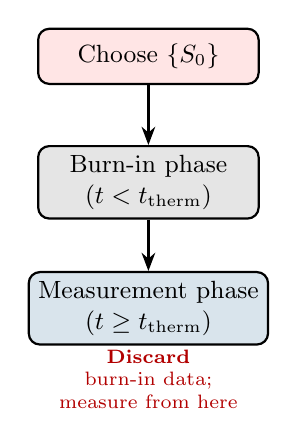
\begin{tikzpicture}[
      box/.style={draw, rounded corners, minimum width=2.8cm, minimum height=0.7cm,
                  text centered, font=\small, thick, align=center},
      arr/.style={-{Stealth}, thick}
    ]
      \node[box, fill=red!10] (init) at (0,3.2) {Choose $\{S_0\}$};
      \node[box, fill=gray!20] (burn) at (0,1.6) {Burn-in phase\\($t < t_{\mathrm{therm}}$)};
      \node[box, fill=mainblue!15] (samp) at (0,0) {Measurement phase\\($t \geq t_{\mathrm{therm}}$)};
      \draw[arr] (init) -- (burn);
      \draw[arr] (burn) -- (samp);
      \node[font=\scriptsize, red!70!black, text width=2.6cm, align=center]
        at (0,-0.9) {\textbf{Discard} burn-in data;\\measure from here};
    \end{tikzpicture}
  \end{columns}
\end{frame}

% ============================================================
\section{Classical Algorithms: Metropolis, SW, and Wolff}
% ============================================================

\begin{frame}{The 2D Ising Model: Testbed for Classical Algorithms}
  \begin{columns}[T]
    \column{0.52\textwidth}
    \begin{block}{Hamiltonian}
      \vspace{-0.5em}
      \[
        \mathcal{H} = -J \sum_{\langle ij \rangle} S_i^z\, S_j^z
      \]
      \vspace{-0.8em}
      \begin{itemize}\small
        \item $S_i^z = \pm 1$ on a 2D square lattice
        \item $J > 0$: ferromagnetic; $J < 0$: antiferromagnetic
      \end{itemize}
    \end{block}
    \vspace{0.3em}
    \begin{block}{With next-nearest-neighbor frustration}
      \vspace{-0.5em}
      \[
        \mathcal{H} = -J \!\sum_{\langle ij \rangle} S_i^z S_j^z + J' \!\sum_{\langle\!\langle ik \rangle\!\rangle} S_i^z S_k^z
      \]
      \vspace{-0.3em}
      {\small $J' > 0$: competing AFM interaction $\Rightarrow$ frustration}
    \end{block}

    \column{0.46\textwidth}
    \centering
    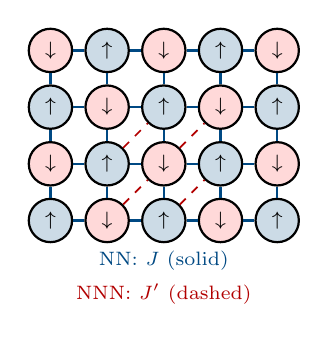
\begin{tikzpicture}[scale=0.72]
      % Spin configuration: alternating pattern
      \foreach \x in {0,...,4}{
        \foreach \y in {0,...,3}{
          \pgfmathtruncatemacro{\parity}{mod(\x+\y,2)}
          \ifnum\parity=0
            \node[circle, draw, thick, minimum size=0.55cm, inner sep=0pt,
                  font=\scriptsize, fill=mainblue!20] (n\x\y) at (\x,\y) {$\uparrow$};
          \else
            \node[circle, draw, thick, minimum size=0.55cm, inner sep=0pt,
                  font=\scriptsize, fill=red!15] (n\x\y) at (\x,\y) {$\downarrow$};
          \fi
        }
      }
      % NN bonds
      \foreach \x in {0,...,4}{
        \foreach \y [evaluate=\y as \yn using int(\y+1)] in {0,...,2}{
          \draw[thick, mainblue] (n\x\y) -- (n\x\yn);
        }
      }
      \foreach \x [evaluate=\x as \xn using int(\x+1)] in {0,...,3}{
        \foreach \y in {0,...,3}{
          \draw[thick, mainblue] (n\x\y) -- (n\xn\y);
        }
      }
      % NNN bonds (diagonal, just a few for illustration)
      \draw[dashed, red!70!black, semithick] (n10) -- (n21);
      \draw[dashed, red!70!black, semithick] (n20) -- (n31);
      \draw[dashed, red!70!black, semithick] (n11) -- (n22);
      \draw[dashed, red!70!black, semithick] (n21) -- (n32);
      % Labels
      \node[font=\scriptsize, mainblue] at (2,-0.7) {NN: $J$ (solid)};
      \node[font=\scriptsize, red!70!black] at (2,-1.3) {NNN: $J'$ (dashed)};
    \end{tikzpicture}
  \end{columns}
\end{frame}

\begin{frame}{Metropolis Algorithm: Single-Spin-Flip}
  \begin{columns}[T]
    \column{0.48\textwidth}
    \begin{block}{Acceptance Probability}
      \vspace{-0.5em}
      \[
        W(S \to S') = \min\!\big(1,\; e^{-\beta \Delta E}\big)
      \]
      \vspace{-0.3em}
      {\small where $\Delta E = E(S') - E(S)$ is the energy change
      from flipping one spin.}
    \end{block}
    \vspace{0.3em}
    \textbf{Properties:}
    \begin{itemize}\small
      \item \textbf{Local} update: flip one spin at a time
      \item Downhill moves ($\Delta E < 0$): always accepted
      \item Uphill moves: accepted with probability $e^{-\beta \Delta E}$
      \item Ergodic: any configuration reachable by sequential flips
    \end{itemize}

    \column{0.50\textwidth}
    \centering
    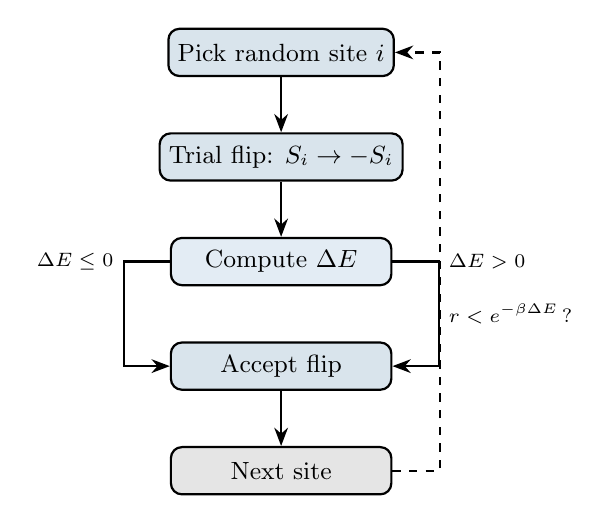
\begin{tikzpicture}[
      box/.style={draw, rounded corners, minimum width=2.8cm, minimum height=0.6cm,
                  text centered, font=\small, thick, align=center},
      arr/.style={-{Stealth}, thick},
      node distance=0.7cm
    ]
      \node[box, fill=mainblue!15] (pick) {Pick random site $i$};
      \node[box, fill=mainblue!15, below=of pick] (flip) {Trial flip: $S_i \to -S_i$};
      \node[box, fill=accentblue!15, below=of flip] (de) {Compute $\Delta E$};
      \node[box, fill=mainblue!15, below=of de] (acc) {Accept flip};
      \node[box, fill=gray!20, below=of acc] (next) {Next site};

      \draw[arr] (pick) -- (flip);
      \draw[arr] (flip) -- (de);
      \draw[arr] (de) -- ++(-2.0,0) node[left, font=\scriptsize] {$\Delta E \leq 0$} |- (acc);
      \draw[arr] (de) -- ++(2.0,0) node[right, font=\scriptsize] {$\Delta E > 0$}
        |- node[near start, right, font=\scriptsize] {$r < e^{-\beta\Delta E}\,$?} (acc);
      \draw[arr] (acc) -- (next);
      \draw[arr, dashed] (next.east) -- ++(0.6,0) |- (pick.east);
    \end{tikzpicture}
  \end{columns}
\end{frame}

\begin{frame}{Metropolis: Detailed Balance Verification}
  \begin{block}{Proof of Detailed Balance}
    For a single spin flip at site $i$, let $S'$ differ from $S$ only at $i$:
    \[
      \frac{W(S \to S')}{W(S' \to S)}
      = \frac{\min\!\big(1,\, e^{-\beta(E_{S'} - E_S)}\big)}
             {\min\!\big(1,\, e^{-\beta(E_S - E_{S'})}\big)}
    \]
    \textbf{Case 1:} $E_{S'} \leq E_S$ \quad$\Rightarrow$\quad
    numerator $= 1$, denominator $= e^{-\beta(E_S - E_{S'})}$
    \[
      \therefore\quad \frac{W(S \to S')}{W(S' \to S)} = e^{-\beta(E_{S'} - E_S)}
      = \frac{\pi(S')}{\pi(S)} \quad\checkmark
    \]
    \textbf{Case 2:} $E_{S'} > E_S$ \quad$\Rightarrow$\quad same result by symmetry.
  \end{block}
  \vspace{0.3em}
  \begin{exampleblock}{Ergodicity}
    Since each spin can be flipped individually, any configuration $\{S\}$ can be transformed into any other $\{S'\}$ by at most $N$ single-spin flips. \quad$\checkmark$
  \end{exampleblock}
\end{frame}

\begin{frame}{Swendsen--Wang Algorithm: Bond Percolation}
  \begin{columns}[T]
    \column{0.48\textwidth}
    \begin{block}{Fortuin--Kasteleyn Bond Activation}
      For each pair of \textbf{aligned} nearest neighbors $S_i = S_j$:
      \[
        p_{\mathrm{bond}} = 1 - e^{-2\beta J}
      \]
      Activate bond with probability $p_{\mathrm{bond}}$; never bond anti-aligned pairs.
    \end{block}
    \vspace{0.3em}
    \textbf{Algorithm:}
    \begin{enumerate}\small
      \item Scan all NN bonds; activate with prob $p_{\mathrm{bond}}$
      \item Identify connected clusters via union-find
      \item Flip each cluster independently with prob $1/2$
    \end{enumerate}

    \column{0.50\textwidth}
    \centering
    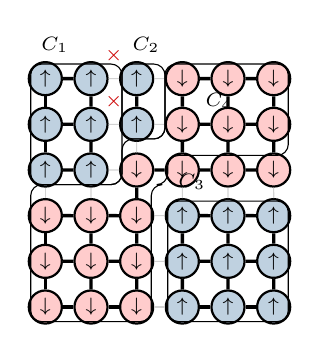
\begin{tikzpicture}[scale=0.58,
      up/.style={circle, draw, thick, fill=mainblue!25, minimum size=0.42cm,
                 inner sep=0pt, font=\scriptsize},
      dn/.style={circle, draw, thick, fill=red!20, minimum size=0.42cm,
                 inner sep=0pt, font=\scriptsize}]
      % 6×6 diagonal domain wall
      % y=0: ↓↓↓↑↑↑    y=1: ↓↓↓↑↑↑    y=2: ↓↓↓↑↑↑
      % y=3: ↑↑↓↓↓↓    y=4: ↑↑↑↓↓↓    y=5: ↑↑↑↓↓↓
      \foreach \x in {0,1,2} { \node[dn] (n\x 0) at (\x,0) {$\downarrow$}; }
      \foreach \x in {3,4,5} { \node[up] (n\x 0) at (\x,0) {$\uparrow$}; }
      \foreach \x in {0,1,2} { \node[dn] (n\x 1) at (\x,1) {$\downarrow$}; }
      \foreach \x in {3,4,5} { \node[up] (n\x 1) at (\x,1) {$\uparrow$}; }
      \foreach \x in {0,1,2} { \node[dn] (n\x 2) at (\x,2) {$\downarrow$}; }
      \foreach \x in {3,4,5} { \node[up] (n\x 2) at (\x,2) {$\uparrow$}; }
      \foreach \x in {0,1}   { \node[up] (n\x 3) at (\x,3) {$\uparrow$}; }
      \foreach \x in {2,...,5}{ \node[dn] (n\x 3) at (\x,3) {$\downarrow$}; }
      \foreach \x in {0,1,2} { \node[up] (n\x 4) at (\x,4) {$\uparrow$}; }
      \foreach \x in {3,4,5} { \node[dn] (n\x 4) at (\x,4) {$\downarrow$}; }
      \foreach \x in {0,1,2} { \node[up] (n\x 5) at (\x,5) {$\uparrow$}; }
      \foreach \x in {3,4,5} { \node[dn] (n\x 5) at (\x,5) {$\downarrow$}; }

      % Background: all NN edges (thin gray)
      \foreach \x in {0,...,5}{
        \foreach \y [evaluate=\y as \yn using int(\y+1)] in {0,...,4}{
          \draw[gray!35] (n\x\y) -- (n\x\yn);
        }
      }
      \foreach \x [evaluate=\x as \xn using int(\x+1)] in {0,...,4}{
        \foreach \y in {0,...,5}{
          \draw[gray!35] (n\x\y) -- (n\xn\y);
        }
      }

      % Active bonds (thick black, following reference style)
      % Cluster 1 (white/up, top-left): (0-1,3)(0-1,4)(0-1,5)
      \draw[line width=1.2pt] (n03) -- (n13);
      \draw[line width=1.2pt] (n03) -- (n04);  \draw[line width=1.2pt] (n04) -- (n05);
      \draw[line width=1.2pt] (n13) -- (n14);  \draw[line width=1.2pt] (n14) -- (n15);
      \draw[line width=1.2pt] (n04) -- (n14);  \draw[line width=1.2pt] (n05) -- (n15);
      % Stochastic miss: (1,4)-(2,4) and (1,5)-(2,5) NOT bonded → isolates col 2 top
      % Cluster 2 (white/up, col 2 top): (2,4)(2,5)
      \draw[line width=1.2pt] (n24) -- (n25);
      % Miss markers
      \node[font=\scriptsize, red!80!black] at (1.5,4.5) {$\times$};
      \node[font=\scriptsize, red!80!black] at (1.5,5.5) {$\times$};

      % Cluster 3 (white/up, bottom-right): (3-5, 0-2)
      \foreach \x [evaluate=\x as \xn using int(\x+1)] in {3,4}{
        \foreach \y in {0,1,2}{
          \draw[line width=1.2pt] (n\x\y) -- (n\xn\y);
        }
      }
      \foreach \x in {3,4,5}{
        \draw[line width=1.2pt] (n\x 0) -- (n\x 1);
        \draw[line width=1.2pt] (n\x 1) -- (n\x 2);
      }

      % Cluster 4 (black/dn, large): bottom-left + top-right via bridge
      % Bottom-left 3×3 block
      \foreach \x [evaluate=\x as \xn using int(\x+1)] in {0,1}{
        \foreach \y [evaluate=\y as \yn using int(\y+1)] in {0,1}{
          \draw[line width=1.2pt] (n\x\y) -- (n\xn\y);
          \draw[line width=1.2pt] (n\x\y) -- (n\x\yn);
        }
      }
      \draw[line width=1.2pt] (n02) -- (n12);  \draw[line width=1.2pt] (n12) -- (n22);
      \draw[line width=1.2pt] (n20) -- (n21);  \draw[line width=1.2pt] (n21) -- (n22);
      % Bridge (2,2)↓–(2,3)↓
      \draw[line width=1.2pt] (n22) -- (n23);
      % Top-right down region
      \draw[line width=1.2pt] (n23) -- (n33);  \draw[line width=1.2pt] (n33) -- (n43);
      \draw[line width=1.2pt] (n43) -- (n53);
      \draw[line width=1.2pt] (n33) -- (n34);  \draw[line width=1.2pt] (n43) -- (n44);
      \draw[line width=1.2pt] (n53) -- (n54);
      \draw[line width=1.2pt] (n34) -- (n44);  \draw[line width=1.2pt] (n44) -- (n54);
      \draw[line width=1.2pt] (n34) -- (n35);  \draw[line width=1.2pt] (n44) -- (n45);
      \draw[line width=1.2pt] (n54) -- (n55);
      \draw[line width=1.2pt] (n35) -- (n45);  \draw[line width=1.2pt] (n45) -- (n55);

      % Cluster outlines (thin black, following reference)
      \draw[thin, rounded corners=4pt]
        (-0.32,2.68) rectangle (1.68,5.32);
      \node[font=\scriptsize, anchor=south west] at (-0.3,5.35) {$C_1$};
      \draw[thin, rounded corners=4pt]
        (1.68,3.68) rectangle (2.62,5.32);
      \node[font=\scriptsize, anchor=south west] at (1.7,5.35) {$C_2$};
      \draw[thin, rounded corners=4pt]
        (2.68,-0.32) rectangle (5.32,2.32);
      \node[font=\scriptsize, anchor=south west] at (2.7,2.35) {$C_3$};
      \draw[thin, rounded corners=4pt]
        (-0.32,-0.32) -- (2.32,-0.32) -- (2.32,2.68) -- (2.68,2.68)
        -- (2.68,3.32) -- (5.32,3.32) -- (5.32,5.32) -- (2.62,5.32)
        -- (2.62,3.68) -- (1.68,3.68) -- (1.68,2.68) -- (-0.32,2.68)
        -- cycle;
      \node[font=\scriptsize] at (3.8,4.5) {$C_4$};
    \end{tikzpicture}
  \end{columns}
\end{frame}

\begin{frame}{Swendsen-Wang Flipping Process}
  \centering
  \vspace{-1em}
  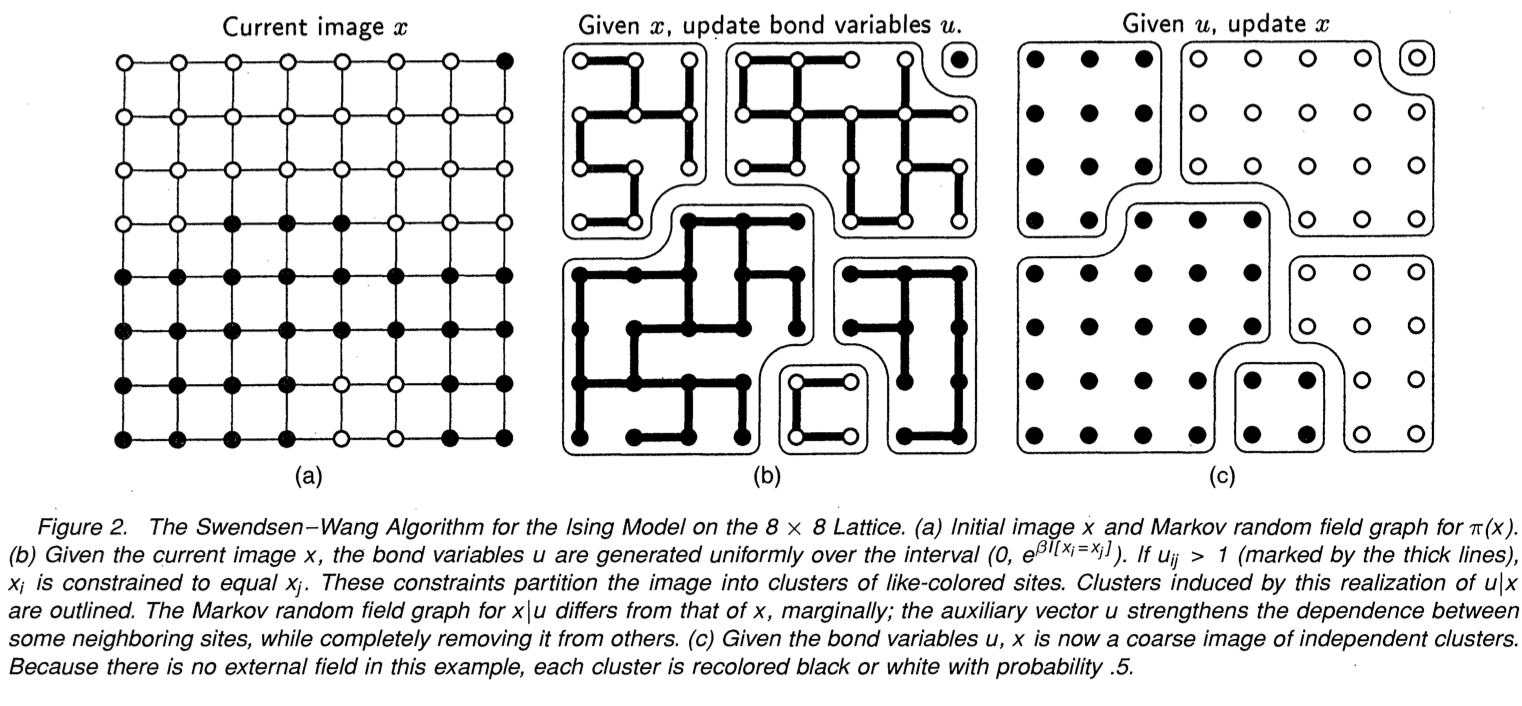
\includegraphics[width=0.9\textwidth,height=0.84\textheight,keepaspectratio]{SW_example2.png}
\end{frame}

\begin{frame}{Swendsen--Wang: Detailed Balance}
  \begin{block}{Transition Probability}
    \vspace{-0.3em}
    {\small Probability to go from $S$ to a specific $S'$:
    \[
      W_{\mathrm{SW}}(S \to S') = \sum_{B\sim S,S'} P(B \mid S)\;\Big(\frac{1}{2}\Big)^{\!N_C(B)}
    \]
    \vspace{-0.5em}
    Sum over bond configs $B$ compatible with both $S$ and $S'$; each of $N_C$ clusters flipped independently with prob $1/2$.}
  \end{block}
  \vspace{0.1em}
  \begin{exampleblock}{Detailed Balance Holds}
    \vspace{-0.3em}
    {\small In the FK representation ($e^{\beta J|E|}$ cancels in the ratio):
    \[
      \frac{W_{\mathrm{SW}}(S \to S')}{W_{\mathrm{SW}}(S' \to S)}
      = \frac{\prod_{\langle ij \rangle} e^{\beta J\,(1 + S'_i S'_j)}}
             {\prod_{\langle ij \rangle} e^{\beta J\,(1 + S_i S_j)}}
      = e^{-\beta(E_{S'} - E_S)}
      = \frac{\pi(S')}{\pi(S)} \quad\checkmark
    \]
    \vspace{-0.3em}
    Key: $p = 1 - e^{-2\beta J}$ is chosen so that $e^{\beta J}(1-p) = e^{-\beta J}$.}
  \end{exampleblock}
  \vspace{0.1em}
  {\small\textbf{Ergodicity:} with prob $(1\!-\!p)^{|E|}\!>\!0$, all bonds absent $\Rightarrow$ $N$ single-site clusters $\Rightarrow$ any config reachable. \;$\checkmark$}
\end{frame}

\begin{frame}{SW Detailed Balance: Full Derivation \textit{(backup)}}
  \begin{columns}[T]
    \column{0.48\textwidth}
    \textbf{Step 1.} Bond probability:
    \vspace{-0.3em}
    \[
      P(B \mid S) = \!\!\prod_{\langle ij \rangle:\, S_i=S_j}
      p^{b_{ij}}(1-p)^{1-b_{ij}}
    \]
    \vspace{-0.5em}
    {\small $b_{ij}\!\in\!\{0,1\}$: bond indicator in $B$; bonds only between aligned spins.}

    \vspace{0.5em}
    \textbf{Step 2.} Boltzmann weight (FK form):
    \vspace{-0.3em}
    \[
      \pi(S) \propto \prod_{\langle ij\rangle} e^{\beta J(1 + S_i S_j)}
    \]
    \vspace{-0.5em}
    {\small $\Rightarrow e^{2\beta J}$ for aligned, $1$ for anti-aligned.}

    \column{0.50\textwidth}
    \textbf{Step 3.} Transition probability:
    \vspace{-0.3em}
    \[
      W_{\mathrm{SW}}(S \to S') = \sum_{B\sim S,S'} P(B\mid S)\;\Big(\frac{1}{2}\Big)^{\!N_C}
    \]

    \vspace{0.5em}
    \textbf{Step 4.} Detailed balance via key lemma\\
    {\small (next slide: $\pi(S)\,P(B|S) = \pi(S')\,P(B|S')$):}
    \vspace{-0.3em}
    \begin{align*}
      \pi(S)\,W(S\!\to\!S')
      &= \textstyle\sum_B \underbrace{\pi(S)\,P(B|S)}_{\displaystyle=\,\pi(S')\,P(B|S')}\,(1/2)^{N_C}\\
      &= \pi(S')\,W(S'\!\to\!S)
    \end{align*}
    \vspace{-0.8em}
    {\small $\Rightarrow\; W(S\!\to\!S')/W(S'\!\to\!S) = \pi(S')/\pi(S)\;\checkmark$}
  \end{columns}
\end{frame}

\begin{frame}{SW Detailed Balance: Why It Really Works \textit{(backup)}}
  \begin{columns}[T]
    \column{0.48\textwidth}
    \textbf{Key lemma.}\; Define $f(S,B) = \pi(S)\cdot P(B\mid S)$:
    \[
      f(S,B) \propto \!\!\prod_{\langle ij \rangle} e^{\beta J S_iS_j}\!
      \cdot p^{b_{ij}}(1\!-\!p)^{1-b_{ij}}
    \]
    {\small Per-bond contribution to $f$:}
    \[
      \begin{cases}
        e^{\beta J}\!\cdot\! p & b_{ij}=1,\; S_i\!=\!S_j \\
        e^{\beta J}\!(1\!-\!p) \stackrel{!}{=} e^{-\beta J} & b_{ij}=0,\; S_i\!=\!S_j \\
        e^{-\beta J} & b_{ij}=0,\; S_i\!\neq\! S_j
      \end{cases}
    \]
    \vspace{-0.5em}
    {\small $e^{\beta J}(1\!-\!p) = e^{-\beta J}$ iff $p = 1\!-\!e^{-2\beta J}$ $\checkmark$}

    \column{0.50\textwidth}
    \textbf{Cluster flip invariance.}

    {\small When cluster $C_k$ flips ($S_i \!\to\! -S_i$ for $i \!\in\! C_k$):}
    \begin{itemize}\small
      \item \textbf{Intra-cluster}: both spins flip $\Rightarrow$ $S_iS_j$ unchanged $\Rightarrow$ contribution unchanged
      \item \textbf{Boundary} ($b_{ij}\!=\!0$, one site in $C_k$): $S_iS_j$ flips sign, but aligned $\leftrightarrow$ anti-aligned both give $e^{-\beta J}$ $\Rightarrow$ unchanged
    \end{itemize}

    \vspace{0.2em}
    $\therefore\; f(S,B) = f(S',B)$ for every compatible $B$.

    \vspace{0.4em}
    \textbf{Detailed balance:}
    \[
      \pi(S)\,W(S\!\to\!S') = \textstyle\sum_B f(S,B)(\tfrac{1}{2})^{N_C}
    \]
    \[
      = \textstyle\sum_B f(S',B)(\tfrac{1}{2})^{N_C} = \pi(S')\,W(S'\!\to\!S)
    \]
  \end{columns}
\end{frame}
\begin{frame}{Wolff Algorithm: Single-Cluster Update}
  \begin{columns}[T]
    \column{0.48\textwidth}
    \begin{block}{Core Idea}
      Instead of building \emph{all} clusters (SW), grow \textbf{one cluster} from a random seed site using the same FK bond probability:
      \[
        p_{\mathrm{bond}} = 1 - e^{-2\beta J}
      \]
    \end{block}
    \vspace{0.2em}
    \textbf{Algorithm:}
    \begin{enumerate}\small
      \item Pick a random seed site $i_0$
      \item For each unvisited neighbor $j$ of the cluster frontier:\\
            if $S_j = S_{i_0}$, add $j$ with prob $p_{\mathrm{bond}}$
      \item Repeat step 2 until no new members
      \item Flip the entire cluster
    \end{enumerate}
    \vspace{0.2em}
    {\footnotesize Ref: U.\ Wolff, PRL \textbf{62}, 361 (1989)}

    \column{0.50\textwidth}
    \centering
    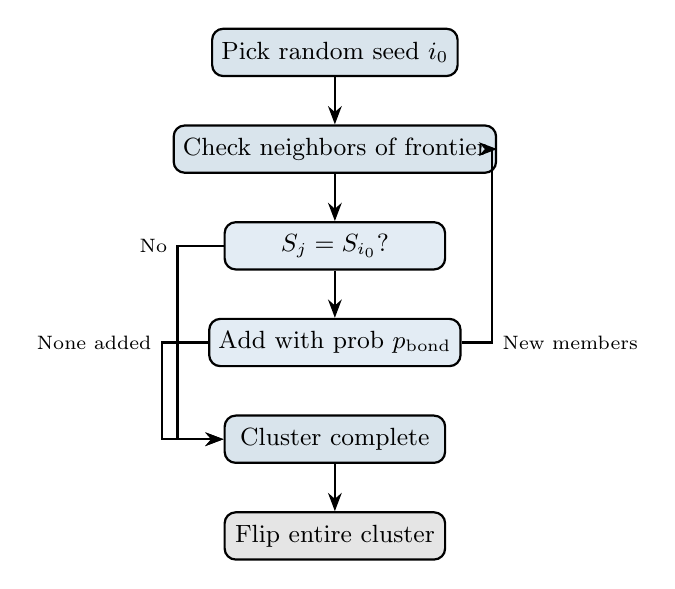
\begin{tikzpicture}[
      box/.style={draw, rounded corners, minimum width=2.8cm, minimum height=0.6cm,
                  text centered, font=\small, thick, align=center},
      arr/.style={-{Stealth}, thick},
      node distance=0.6cm
    ]
      \node[box, fill=mainblue!15] (seed) {Pick random seed $i_0$};
      \node[box, fill=mainblue!15, below=of seed] (frontier) {Check neighbors of frontier};
      \node[box, fill=accentblue!15, below=of frontier] (bond) {$S_j = S_{i_0}$?};
      \node[box, fill=accentblue!15, below=of bond] (prob) {Add with prob $p_{\mathrm{bond}}$};
      \node[box, fill=mainblue!15, below=of prob] (done) {Cluster complete};
      \node[box, fill=gray!20, below=of done] (flip) {Flip entire cluster};

      \draw[arr] (seed) -- (frontier);
      \draw[arr] (frontier) -- (bond);
      \draw[arr] (bond) -- ++(-2.0,0) node[left, font=\scriptsize] {No} |- (done);
      \draw[arr] (bond) -- (prob);
      \draw[arr] (prob) -- ++(2.0,0) node[right, font=\scriptsize] {New members} |- (frontier.east);
      \draw[arr] (prob) -- ++(-2.2,0) node[left, font=\scriptsize] {None added} |- (done.west);
      \draw[arr] (done) -- (flip);
    \end{tikzpicture}
  \end{columns}
\end{frame}

\begin{frame}{Wolff: Cluster Growth Example}
  \centering
  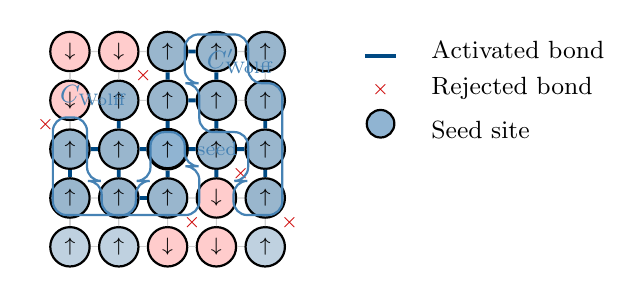
\begin{tikzpicture}[scale=0.62,
    up/.style={circle, draw, thick, minimum size=0.5cm, inner sep=0pt,
               font=\scriptsize},
    dn/.style={circle, draw, thick, minimum size=0.5cm, inner sep=0pt,
               font=\scriptsize}]
    % 5×5 lattice — most spins up, a few down
    % Row 0: ↑↑↓↓↑
    \node[up, fill=mainblue!25] (n00) at (0,0) {$\uparrow$};
    \node[up, fill=mainblue!25] (n10) at (1,0) {$\uparrow$};
    \node[dn, fill=red!20]      (n20) at (2,0) {$\downarrow$};
    \node[dn, fill=red!20]      (n30) at (3,0) {$\downarrow$};
    \node[up, fill=mainblue!25] (n40) at (4,0) {$\uparrow$};
    % Row 1: ↑↑↑↓↑
    \node[up, fill=mainblue!40] (n01) at (0,1) {$\uparrow$};
    \node[up, fill=mainblue!40] (n11) at (1,1) {$\uparrow$};
    \node[up, fill=mainblue!40] (n21) at (2,1) {$\uparrow$};
    \node[dn, fill=red!20]      (n31) at (3,1) {$\downarrow$};
    \node[up, fill=mainblue!40] (n41) at (4,1) {$\uparrow$};
    % Row 2: ↑↑↑↑↑  (seed in center)
    \node[up, fill=mainblue!40] (n02) at (0,2) {$\uparrow$};
    \node[up, fill=mainblue!40] (n12) at (1,2) {$\uparrow$};
    \node[up, fill=accentblue!60, line width=1.2pt] (n22) at (2,2) {$\uparrow$};
    \node[up, fill=mainblue!40] (n32) at (3,2) {$\uparrow$};
    \node[up, fill=mainblue!40] (n42) at (4,2) {$\uparrow$};
    % Row 3: ↓↑↑↑↑
    \node[dn, fill=red!20]      (n03) at (0,3) {$\downarrow$};
    \node[up, fill=mainblue!40] (n13) at (1,3) {$\uparrow$};
    \node[up, fill=mainblue!40] (n23) at (2,3) {$\uparrow$};
    \node[up, fill=mainblue!40] (n33) at (3,3) {$\uparrow$};
    \node[up, fill=mainblue!40] (n43) at (4,3) {$\uparrow$};
    % Row 4: ↓↓↑↑↑
    \node[dn, fill=red!20]      (n04) at (0,4) {$\downarrow$};
    \node[dn, fill=red!20]      (n14) at (1,4) {$\downarrow$};
    \node[up, fill=mainblue!40] (n24) at (2,4) {$\uparrow$};
    \node[up, fill=mainblue!40] (n34) at (3,4) {$\uparrow$};
    \node[up, fill=mainblue!40] (n44) at (4,4) {$\uparrow$};

    % All NN edges (thin gray)
    \foreach \x in {0,...,4}{
      \foreach \y [evaluate=\y as \yn using int(\y+1)] in {0,...,3}{
        \draw[gray!35] (n\x\y) -- (n\x\yn);
      }
    }
    \foreach \x [evaluate=\x as \xn using int(\x+1)] in {0,...,3}{
      \foreach \y in {0,...,4}{
        \draw[gray!35] (n\x\y) -- (n\xn\y);
      }
    }

    % Seed marker
    \node[font=\scriptsize, accentblue, anchor=west] at (2.4,2.0) {seed};

    % Activated bonds (thick, in cluster)
    % From seed (2,2): activate to (1,2), (3,2), (2,1), (2,3)
    \draw[line width=1.4pt, mainblue] (n22) -- (n12);
    \draw[line width=1.4pt, mainblue] (n22) -- (n32);
    \draw[line width=1.4pt, mainblue] (n22) -- (n21);
    \draw[line width=1.4pt, mainblue] (n22) -- (n23);
    % From (1,2): activate to (0,2), (1,1), (1,3)
    \draw[line width=1.4pt, mainblue] (n12) -- (n02);
    \draw[line width=1.4pt, mainblue] (n12) -- (n11);
    \draw[line width=1.4pt, mainblue] (n12) -- (n13);
    % From (3,2): activate to (4,2), (3,1), (3,3)
    \draw[line width=1.4pt, mainblue] (n32) -- (n42);
    \draw[line width=1.4pt, mainblue] (n32) -- (n31);
    \draw[line width=1.4pt, mainblue] (n32) -- (n33);
    % From (2,1): activate to (1,1), (2,0 rejected — ↓)
    % (1,1) already connected via (1,2); (2,1)-(1,1) bond:
    \draw[line width=1.4pt, mainblue] (n21) -- (n11);
    % From (2,1): bond to (3,1) rejected (↓)
    \node[font=\scriptsize, red!80!black] at (2.5,0.5) {$\times$};
    \node[font=\scriptsize, red!80!black] at (3.5,1.5) {$\times$};
    % From (2,3): activate to (3,3), (2,4)
    % (3,3) already via (3,2)
    \draw[line width=1.4pt, mainblue] (n23) -- (n33);
    \draw[line width=1.4pt, mainblue] (n23) -- (n24);
    % From (2,3): bond to (1,3) rejected (stochastic miss)
    \node[font=\scriptsize, red!80!black] at (1.5,3.5) {$\times$};
    % From (0,2): activate to (0,1)
    \draw[line width=1.4pt, mainblue] (n02) -- (n01);
    % From (0,2): bond to (0,3) rejected (↓)
    \node[font=\scriptsize, red!80!black] at (-0.5,2.5) {$\times$};
    % From (4,2): activate to (4,1), (4,3)
    \draw[line width=1.4pt, mainblue] (n42) -- (n41);
    \draw[line width=1.4pt, mainblue] (n42) -- (n43);
    % From (4,1): bond to (4,0) rejected (stochastic)
    \node[font=\scriptsize, red!80!black] at (4.5,0.5) {$\times$};
    % From (3,3): activate to (3,4)
    \draw[line width=1.4pt, mainblue] (n33) -- (n34);
    % From (2,4): activate to (3,4)
    \draw[line width=1.4pt, mainblue] (n24) -- (n34);

    % Cluster outline
    \draw[thick, rounded corners=5pt, accentblue]
      (-0.35,0.65) -- (-0.35,2.65) -- (0.35,2.65) -- (0.35,1.35)
      -- (0.65,1.35) -- (0.65,0.65) -- (1.35,0.65) -- (1.35,1.35)
      -- (1.65,1.35) -- (1.65,2.35) -- (2.35,2.35) -- (2.35,1.65)
      -- (2.65,1.65) -- (2.65,0.65) -- cycle;
    \node[font=\small, accentblue, anchor=south west] at (-0.4,2.7) {$C_{\mathrm{Wolff}}$};

    % Second cluster outline (right side)
    \draw[thick, rounded corners=5pt, accentblue]
      (2.65,2.35) -- (2.65,3.35) -- (2.35,3.35) -- (2.35,4.35)
      -- (3.65,4.35) -- (3.65,3.35) -- (4.35,3.35) -- (4.35,0.65)
      -- (3.35,0.65) -- (3.35,1.35) -- (3.65,1.35) -- (3.65,2.35)
      -- cycle;
    \node[font=\small, accentblue] at (3.5,3.8) {$C'_{\mathrm{Wolff}}$};

    % Legend
    \node[font=\small, anchor=north west] at (5.8,4.5) {%
      \begin{tabular}{@{}cl@{}}
        \tikz\draw[line width=1.4pt,mainblue](0,0)--(0.4,0); & Activated bond \\[2pt]
        {\scriptsize\color{red!80!black}$\times$} & Rejected bond \\[2pt]
        \tikz\node[circle,draw,thick,fill=accentblue!60,minimum size=0.35cm,inner sep=0pt]{}; & Seed site \\
      \end{tabular}};
  \end{tikzpicture}
\end{frame}

\begin{frame}{Wolff: Detailed Balance}
  \begin{block}{Transition Probability}
    {\small $W(S \to S') \neq 0$ only when $S'$ is obtained by flipping \textbf{one} connected cluster $C$ of aligned spins. For such a pair:
    $\;W_{\mathrm{Wolff}}(S \to S') = \dfrac{|C|}{N}\;\displaystyle\prod_{\mathcal{I}(C)}\!p\;\displaystyle\prod_{\substack{\partial C \\ S_i=S_j}}\!(1-p)$}\\[3pt]
    {\footnotesize $|C|/N$: seed in $C$;\quad $\mathcal{I}(C)$: internal bonds activated;\quad $\partial C$: boundary bonds rejected (stop growth).}
  \end{block}
  \begin{exampleblock}{Detailed Balance}
    {\small $|C|/N$ and $\prod_{\mathcal{I}} p$ cancel in ratio (same cluster, same internal bonds).
    Only $\partial C$ contributes:
    \[
      \frac{W(S \to S')}{W(S' \to S)}
      = \prod_{\substack{\langle ij \rangle \in \partial C \\ S_i = S_j}}\!\frac{(1-p)}{1}
      \;\cdot\prod_{\substack{\langle ij \rangle \in \partial C \\ S_i \neq S_j}}\!\frac{1}{(1-p)}
    \]}
    {\footnotesize After flip: aligned $\leftrightarrow$ anti-aligned swap on $\partial C$.
    With $(1-p) = e^{-2\beta J}$: $\;\dfrac{W(S \to S')}{W(S' \to S)} = e^{-\beta(E_{S'}-E_S)} = \dfrac{\pi(S')}{\pi(S)}\;\checkmark$}
    \vspace{0.2em}

    {\small \textbf{Ergodicity:} cluster of size 1 (all bonds reject) $\Rightarrow$ single spin flip. $\checkmark$}
  \end{exampleblock}
\end{frame}

\begin{frame}{Wolff Detailed Balance: Full Derivation \textit{(backup)}}
  {\small\textbf{Key difference from SW:} one Wolff step flips only \emph{one} cluster $C$.
  $W(S\!\to\!S') = 0$ unless $S'$ differs from $S$ by flipping a single connected cluster.
  Arbitrary $S \to S'$ may need \emph{multiple} Wolff steps — but detailed balance is checked per step.}
  \begin{columns}[T]
    \column{0.48\textwidth}
    \textbf{Step 1.} For $S'$ reachable via cluster $C$:
    \vspace{-0.3em}
    \[
      W(S\!\to\!S') = \frac{|C|}{N}\prod_{\mathcal{I}(C)}\!p
          \prod_{\substack{\langle ij\rangle\in\partial C\\S_i=S_j}}\!(1\!-\!p)
    \]
    \vspace{-0.5em}
    {\small $\frac{|C|}{N}$: seed in $C$;\; $\mathcal{I}(C)$: activated;\; $\partial C$: rejected.}

    \vspace{0.3em}
    \textbf{Step 2.} Cancel common factors:
    \vspace{-0.2em}
    \[
      \frac{W(S\!\to\!S')}{W(S'\!\to\!S)} = \frac{\prod_{\partial,\,S_i=S_j}(1\!-\!p)}{\prod_{\partial,\,S'_i=S'_j}(1\!-\!p)}
    \]
    \vspace{-0.5em}
    {\small $|C|/N$ cancels (same $C$); $\prod_{\mathcal{I}} p$ cancels.}

    \column{0.50\textwidth}
    \textbf{Step 3.} Boundary bond contributions:\\
    {\small Each boundary bond ($i\!\in\!C$, $j\!\notin\!C$) contributes differently:}
    \vspace{0.2em}

    {\footnotesize
    \begin{tabular}{@{}lccc@{}}
      \toprule
      Bond in $S$ & $W(S\!\to\!S')$ & In $S'$ & $W(S'\!\to\!S)$ \\
      \midrule
      Aligned & $(1\!-\!p)$ {\tiny(reject)} & Anti-aligned & $1$ {\tiny(no check)} \\
      Anti-aligned & $1$ {\tiny(no check)} & Aligned & $(1\!-\!p)$ {\tiny(reject)} \\
      \bottomrule
    \end{tabular}}
    \vspace{0.3em}

    {\small After flip: aligned $\leftrightarrow$ anti-aligned swap $\Rightarrow$ contributions also swap.}
  \end{columns}
\end{frame}

\begin{frame}{Wolff: Verify Detailed Balance \textit{(backup, cont.)}}
  \begin{columns}[T]
    \column{0.48\textwidth}
    \textbf{Step 4.} Substitute $1-p = e^{-2\beta J}$:
    \[
      \frac{W(S\!\to\!S')}{W(S'\!\to\!S)}
      = \!\!\prod_{\substack{\partial C\\ S_i=S_j}}\! e^{-2\beta J}
      \cdot \prod_{\substack{\partial C\\ S_i\neq S_j}}\! e^{2\beta J}
    \]

    {\small Let $n_\uparrow$ = aligned boundary bonds, $n_\downarrow$ = anti-aligned:
    \[
      = (e^{-2\beta J})^{n_\uparrow}\!(e^{2\beta J})^{n_\downarrow}
      = e^{-2\beta J(n_\uparrow - n_\downarrow)}
    \]}

    \column{0.50\textwidth}
    \textbf{Step 5.} Energy change on $\partial C$:
    {\small
    \begin{align*}
      E_S\big|_{\partial C} &= -J\,n_\uparrow + J\,n_\downarrow \\
      E_{S'}\big|_{\partial C} &= -J\,n_\downarrow + J\,n_\uparrow
    \end{align*}
    \vspace{-0.8em}

    (aligned $\leftrightarrow$ anti-aligned swap after flip)}\\[4pt]
    {\small $\Delta E = E_{S'} - E_S = 2J(n_\uparrow - n_\downarrow)$}
    \vspace{0.2em}

    \begin{exampleblock}{Conclusion}
      \vspace{-0.3em}
      \[
        e^{-\beta\Delta E} = e^{-2\beta J(n_\uparrow - n_\downarrow)} = \frac{W(S\!\to\!S')}{W(S'\!\to\!S)}\;\checkmark
      \]
      \vspace{-0.8em}
    \end{exampleblock}
  \end{columns}
\end{frame}

\begin{frame}{Comparison: Metropolis vs.\ SW vs.\ Wolff}
  \centering
  \vspace{-0.3em}
  \begin{tabular}{@{}lccc@{}}
    \toprule
    & \textbf{Metropolis} & \textbf{Swendsen--Wang} & \textbf{Wolff} \\
    \midrule
    Update scope & Single spin & All clusters & One cluster \\
    Clusters/sweep & $N$ (trivial) & $\sim N$ & $1$ \\
    Dynamic exp.\ $z$ & $\approx 2$ & $\approx 0.35$ & $\approx 0.25$ \\
    Cost/flip & $O(1)$ & $O(N)$ & $O(\langle|C|\rangle)$ \\
    Best for & Generic models & Frustrated systems & Ferromagnets \\
    \bottomrule
  \end{tabular}
  \vspace{0.5em}

  \begin{columns}[T]
    \column{0.50\textwidth}
    \begin{itemize}\small
      \item \textbf{Metropolis}: simplest; universal but suffers \emph{critical slowing down} ($z \approx 2$)
      \item \textbf{SW}: global update via FK percolation; eliminates most critical slowing down
    \end{itemize}
    \column{0.50\textwidth}
    \begin{itemize}\small
      \item \textbf{Wolff}: single-cluster variant; even lower $z$ than SW for ferromagnets
      \item All three satisfy detailed balance \& ergodicity
      \item Near $T_c$: Wolff is typically the most \emph{efficient per unit cost}
    \end{itemize}
  \end{columns}
\end{frame}

% ============================================================
\section{Wolff Algorithm on Infinite Lattice}
% ============================================================
\begin{frame}{}
  \centering\textit{(Section 5 — to be written)}
\end{frame}

% ============================================================
\section{Loop and Worm Algorithms for Quantum Systems}
% ============================================================
\begin{frame}{}
  \centering\textit{(Section 6 — to be written)}
\end{frame}

% ============================================================
\section{Summary and Outlook}
% ============================================================
\begin{frame}{}
  \centering\textit{(Section 7 — to be written)}
\end{frame}

\end{document}
